\documentclass[]{beamer}
\usepackage[utf8]{inputenc}
\usepackage{graphicx}
\usepackage{subfigure}
\usepackage{varioref}
\usepackage{pgfpages}

\mode<handout>{
    \pgfpagesuselayout{16 on 1}[a0paper]
}

\providecommand{\keywords}[1]{
    \small
    \textbf{Keywords: } #1
}

\title{Intelligent Linguistic System for the Grammar of the Romanian Language}
\subtitle{EEML Summer School 2021 - Virtual Budapest, Hungary}
\author{Ioan Florin Cătălin Nițu, Traian Eugen Rebedea}
\institute{University Politehnica of Bucharest}
\date{June - July 2020}

\bibliographystyle{apalike}

\begin{document}
    
    \begin{frame}
        
        \maketitle
        
    \end{frame}
    
    \begin{abstract}
        
        The proposed correction system receives a sentence with grammatical errors and corrects it, using state-of-the-art technologies to perform this operation such as attention-based Transformers. The paper uses RONACC, the first corpus for grammatical corrections in Romanian for modeling, training, testing, and validating the project. Using a very large data set with over a million learning examples, an average BLEU score of 45.29 points was obtained, in a rather short training time (only two hours for 5 epochs) executed on several GPUs. However, even a small data set of only fifty thousand examples with as many as one hundred epochs achieves an average BLEU score of 33.29 points in three hours. \cite{nitu2020intelligent}
        
        \keywords{Romanian language, grammar, transformers, attention, positional encoding}
        
    \end{abstract}
    
    \begin{frame}
        
        \begin{figure}[]
            \centering
            \includegraphics[width=1.0\textwidth]{teaser.png}
            \label{fig:teaser}
        \end{figure}
        
    \end{frame}
    
    
    \begin{frame}{Outline}
        \tableofcontents
        
    \end{frame}
    
    \section{Introduction}
        
        \begin{frame}{Motivation}
            
            Correcting texts and natural language, in general, is often encountered in computer science, artificial intelligence, and machine learning. The study of natural language processing has brought technologies, models, and products that can competitively address this issue.
            
        \end{frame}
        
    \section{Related Work}
        
        \begin{frame}{Technologies Used}
            
            Python and TensorFlow to implement a Transformer-based solution proposed in the article Attention Is All You Need \cite{vaswani2017attention}:
            \begin{itemize}
                \item Attention layers
                \item Encoder-Decoder Transformer
            \end{itemize}
        
        \end{frame}
        
    \section{Method}
        
        \begin{frame}{Proposed Method}
            
            The data set: RONACC corpus (pairs of lines of correct and wrong sentences).
            
            Training is done in several epochs. The model is not pre-trained.
            
            The transformer is an auto-regressive model \cite{graves2013generating}.
            
            As the transformer predicts each word, attention allows it to look at the previous ones in the input sequence to predict the next one \cite{tensorflow2019transformer}.
        
        \end{frame}
        
    \section{Experiments}
        
        \begin{frame}{RONACC}
            
            Data sets for:
            \begin{itemize}
                \item training:
                \begin{itemize}
                    \item small: 7082 pairs of sentences
                    \item medium: 7082 + 50000 pairs of sentences
                    \item large: 7082 + 1000000 pairs of sentences
                \end{itemize}
                \item testing: 1519 pairs of sentences
                \item validation: 1518 pairs of sentences
            \end{itemize}
            
        \end{frame}
        
        \begin{frame}{Training}
            
            Trained 100 epochs on the (small and) medium data set, testing and measuring accuracy (see Figure \ref{fig:accuracy}) and loss (see Figure \ref{fig:loss}).
            
            \begin{figure}[]
                \centering
                \subfigure[Accuracy]{
                    \centering
                    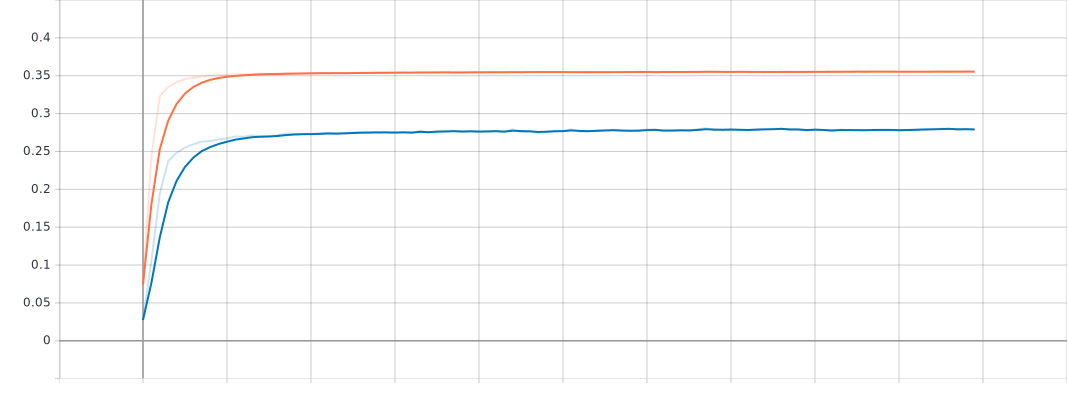
\includegraphics[width=0.45\textwidth]{../../References/medium/accuracy.png}
                    \label{fig:accuracy}
                }
                \hfill
                \subfigure[Loss]{
                    \centering
                    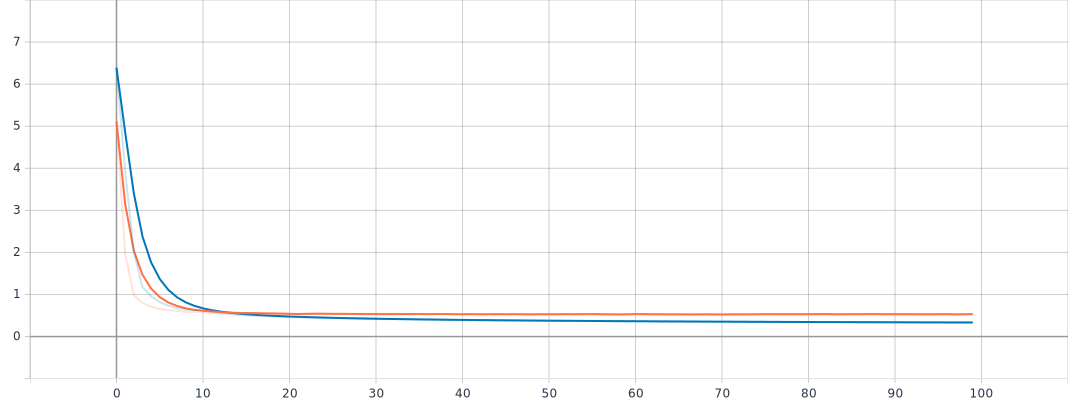
\includegraphics[width=0.45\textwidth]{../../References/medium/loss.png}
                    \label{fig:loss}
                }
                \caption{Metrics for the medium data set}
                \label{fig:metrics}
            \end{figure}
            
        \end{frame}
        
        \begin{frame}{Evaluation}
            
            The model implemented in the presented work obtained a competitive BLEU score of 20.56 for text corrections in Romanian with a modest training set. With an increased training set, it got a score of 33.29, as shown in Table \ref{tab:training-results}, representing a substantial improvement.
            
            \begin{table}[h]
                \caption{Training results}
                \label{tab:training-results}
                \centering
                \begin{tabular}{|c|c|c|c|}
                    \hline
                    Data set & Epochs & BLEU Score & Training time     \\
                    \hline
                    Small    & 100    & 20.56      & 9.66 sec. / epoch \\
                    \hline
                    Medium   & 100    & 33.29      & 99 sec. / epoch   \\
                    \hline
                    Large    & 5      & 45.29      & 1032 sec. / epoch \\
                    \hline
                \end{tabular}
            \end{table}
            
        \end{frame}
        
    \section{Interpretation of the Results}
        
        \begin{frame}{Example Attention (1)}
            
            \begin{columns}
                \column{0.5\textwidth}
                    \begin{itemize}
                        \item Input: Cea mai importantă este \textbf{ceea} surprinsă asupra \textbf{luni} Noiembrie.
                        \item Predicted correction: Cea mai importantă este \textbf{cea} surprinsă asupra \textbf{lunii} Noiembrie.
                        \item Real correction: Cea mai importantă este \textbf{cea} surprinsă asupra \textbf{lunii} Noiembrie.
                    \end{itemize}
                \column{0.5\textwidth}
                    \begin{figure}[htbp]
                        \centering
                        \subfigure[BLEU score: 1.0000]{
                            \centering
                            \includegraphics[width=1.0\textwidth]{../../References/medium/2.png}
                            \label{fig:2}
                        }
                        \caption{Fully Corrected}
                        \label{fig:attention-examples-1}
                    \end{figure}
            \end{columns}
        
        \end{frame}
        
        \begin{frame}{Example Attention (2)}
            
            \begin{columns}
                \column{0.5\textwidth}
                    \begin{itemize}
                        \item Input: În prezent, satul are 3.897 locuitori, \textbf{prepoderent} ucraineni.
                        \item Predicted correction: În prezent, satul are 3.897 locuitori, \textbf{prepoderent} ucraineni.
                        \item Real correction: În prezent, satul are 3.897 locuitori, \textbf{preponderent} ucraineni.
                    \end{itemize}
                \column{0.5\textwidth}
                    \begin{figure}[htbp]
                        \centering
                        \subfigure[BLEU score: 0.7071]{
                            \centering
                            \includegraphics[width=1.0\textwidth]{../../References/medium/5.png}
                            \label{fig:5}
                        }
                        \caption{Partialy Corrected}
                        \label{fig:attention-examples-2}
                    \end{figure}
            \end{columns}
        
        \end{frame}
        
        \begin{frame}{Example Attention (3)}
            
            \begin{columns}
                \column{0.5\textwidth}
                    \begin{itemize}
                        \item Input: „\textbf{Nici odată} \textbf{nam} văzut cartea așa” a mărturisit el.
                        \item Predicted correction: „\textbf{Nici odată} \textbf{nam} văzut cartea așa” a mărturisit el.
                        \item Real correction: „\textbf{Niciodată} \textbf{n-am} văzut cartea așa”, a mărturisit el.
                    \end{itemize}
                \column{0.5\textwidth}
                    \begin{figure}[htbp]
                        \centering
                        \subfigure[BLEU score: 0.2741]{
                            \centering
                            \includegraphics[width=1.0\textwidth]{../../References/medium/3.png}
                            \label{fig:3}
                        }
                        \caption{Sentence with Errors or that Could Not be Corrected}
                        \label{fig:attention-examples-3}
                    \end{figure}
            \end{columns}
        
        \end{frame}
        
    \section{Conclusion}
        
        \begin{frame}{Conclusions}
            
            \begin{itemize}
                \item Model proposed in "Attention Is All You Need" \cite{vaswani2017attention}:
                \begin{itemize}
                    \item trained twelve hours on eight P100 GPUs
                \end{itemize}
                \item Implemented model:
                \begin{itemize}
                    \item on the medium data set: for almost three hours
                    \item on the large set: for an hour and a half (only five epochs)
                \end{itemize}
            \end{itemize}
            Unfortunately, the field development did not make it possible to compare the implemented model with other models.
            This implementation:
            \begin{itemize}
                \item is a starting point in field development
                \item can be used in the construction and modeling of high-performance competitive technologies for text corrections in Romanian
            \end{itemize}
        
        \end{frame}
        
    \begin{frame}{Bibliography}
        
        \bibliography{bibliography}
        
    \end{frame}
    
    \begin{frame}{Thank you for your attention!}
        
        \begin{center}
            ioan\_florin.nitu@stud.acs.upb.ro
        \end{center}

    \end{frame}
    
\end{document}
